\documentclass[letterpaper, 12pt]{article}

\usepackage{geometry}
 \geometry{
 letterpaper,
 total={170mm,257mm},
 left=20mm,
 top=20mm,
 bottom=20mm
 }
\usepackage{graphicx} % Required for inserting images
\usepackage{authblk}
\usepackage{amssymb}
\usepackage{lipsum}
\usepackage{float}
\usepackage{times}
\usepackage{amsmath}
\usepackage[format=plain,
            labelfont={bf,it},
            textfont=it]{caption}
\captionsetup{justification=raggedright,singlelinecheck=false}
\usepackage{ragged2e}
\usepackage{longtable}
\usepackage{comment}
\usepackage{setspace}
\usepackage{fancyhdr}
\usepackage{titlesec}
\usepackage[hyperindex,breaklinks]{hyperref}
\hypersetup{
    colorlinks=true,
    linkcolor=blue,
    filecolor=magenta,      
    urlcolor=blue,
    pdftitle={Overleaf Example},
    pdfpagemode=FullScreen,
    }
% \usepackage{background} % add COSIG logo to page
\usepackage[T1]{fontenc}
\usepackage{helvet}
\renewcommand{\familydefault}{\sfdefault}
\pagenumbering{gobble}
\usepackage[skip=10pt plus1pt, indent=40pt]{parskip}

\begin{comment}
\backgroundsetup{
   scale=1,
   angle=0,
   opacity=1,
   color=black,
   contents={\begin{tikzpicture}[remember picture, overlay]
      \node at ([xshift=3cm,yshift=1cm] current page.south west)
            {
\includegraphics[width = 5cm]{img/home/241017_final_logo_mockup.png}}; %<- change the name of image
     \end{tikzpicture}}
 }
\end{comment}

\titlespacing*{\section}
{0pt}{1.5ex plus 1ex minus .2ex}{1.3ex plus .2ex}

\renewcommand\Authfont{\fontsize{12}{14.4}\selectfont}
\renewcommand\Affilfont{\fontsize{9}{10.8}\itshape}
 
\begin{document}
\flushleft

\includegraphics[width=0.5\textwidth]{img/home/241017_final_logo_mockup.png}

\section*{Standard deviation versus standard error}
\addcontentsline{toc}{section}{Standard deviation versus standard error}
\textit{Last updated: 6 February 2025}

\subsection*{Standard deviation}

\href{https://en.wikipedia.org/wiki/Standard_deviation}{Standard deviation (SD)} is a statistical measure that describes the variability of numerical observations of a variable around the mean of these observations.

When an entire population is measured, the population standard deviation is calculated $\sigma$ is calculated as 

$$
\sigma = \sqrt{\frac{\sum(x_i - \bar{x})^2}{N}}
$$

where $x_i$ is the value of each observation, $\bar{x}$ is the mean of each observation ($\bar{x} = \sum x_i / N$) and $N$ is the number of observations (i.e., the sample size). A lower standard deviation indicates that the data is more closely clustered around its mean, whereas a higher standard deviation indicates that the data is more spread out from its mean.

Note that standard deviation is calculated differently depending on whether you are measuring standard deviation for a population versus just a sample from that population. When only a sample is taken from a population, the sample standard deviation $s$ is calculated as 

$$
s = \sqrt{\frac{\sum(x_i - \bar{x})^2}{N-1}}.
$$

See \href{https://digitalcommons.unl.edu/cgi/viewcontent.cgi?article=1008&context=imseteach}{this explanation by Dr. Paul Savory} for why this correction is made. Most research does not survey a whole population, and thus ``standard deviation" usually denotes sample standard deviation $s$ and not population standard deviation $\sigma$.

Imagine that we took a sample of ten individuals and measured their height in centimeters, obtaining ten observations: 176, 171, 159, 168, 185, 193, 174, 171, 168 and 189. The mean of this sample would be 175.4 and the sample standard deviation would be approximately 10.6.

\subsection*{Standard error}

\href{https://en.wikipedia.org/wiki/Standard_error}{Standard error (SE)} is a measure of the variability of an estimate. For instance, for the previous scenario, a different sample of ten individuals would likely yield a slightly different mean height. The standard error $SE$ is calculated as

$$
SE = \frac{s}{\sqrt{N}}.
$$

Note that as sample size $N$ increases, the standard error decreases. For instance, the mean heights calculated from two different samples of 100 from the same population would likely be closer together than the mean heights calculated from two different samples of only 10. This is why studies with a larger sample size are generally considered more rigorous; their estimates will be more precise. For the previously-listed sample of heights, the standard error of the mean (SEM) would be $10.6/\sqrt{10} \approx 3.3$.

\subsection*{Reporting of standard deviation versus standard error}

When reading a scientific publication, one should take note of whether the authors are reporting variability in their data as standard deviation or standard error. Misidentifying which measure is being reported can give the reader an unrealistic picture of the variability in data and the uncertainty of estimates. There is some evidence that using one measure or the other graphically can lead to this same misinterpretation, even when the reader is aware of which measure is being used (see \href{https://doi.org/10.1073/pnas.2302491120}{Zhang et al., 2023}).

\begin{figure}[h!tbp]
    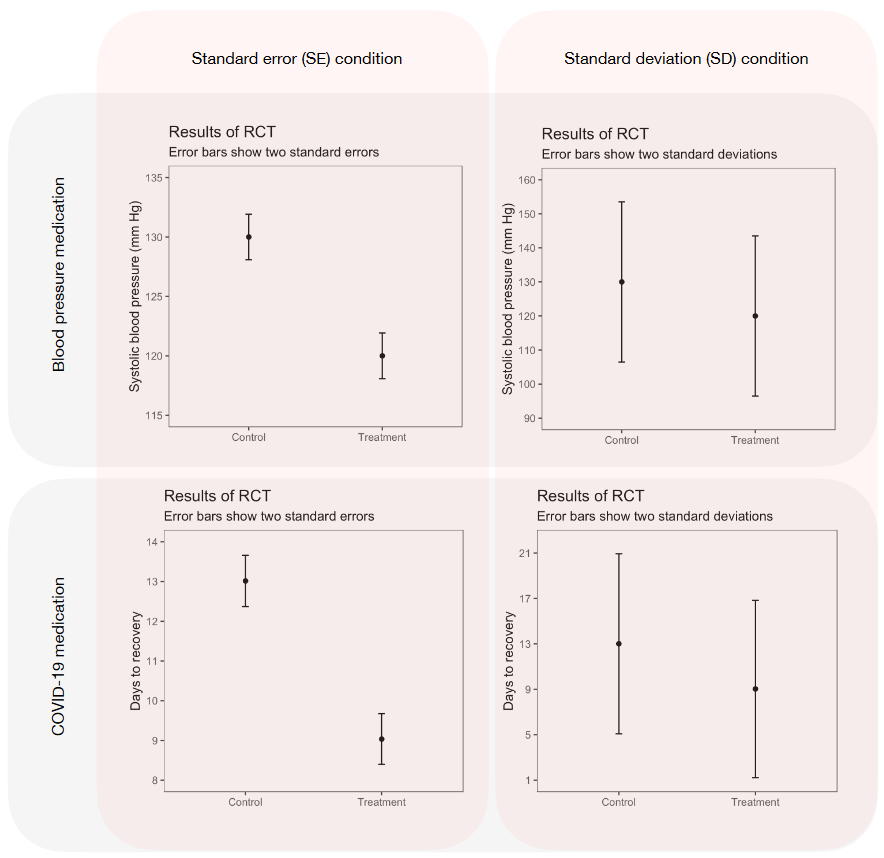
\includegraphics[width=\textwidth]{img/sd_vs_se/zhang_se_vs_sd.png}
    \caption*{Within each row, both charts demonstrate the same hypothetical data from a randomized controlled trial (for blood pressure medication, top row, or COVID-19 medication, bottom row). However, the left charts use error bars to display standard error of the mean and the right charts use error bars to display standard deviation. Adapted from Figure S1 of \href{https://doi.org/10.1073/pnas.2302491120}{Zhang et al. ( 2023)}.}
\end{figure}

\pagebreak

\subsection*{Incorporating variability into a meta-analysis}

A \href{https://en.wikipedia.org/wiki/Meta-analysis}{meta-analysis} is a study that synthesizes the results of independent studies on the same topic to obtain more precise estimates. For instance, one might perform a meta-analysis of randomized controlled trials that all tested the same drug to more precisely determine how effective the drug is at preventing intensive care unit admission or mortality due to COVID-19.

Because larger studies give more precise estimates, they are usually given more weight in meta-analyses so that their findings contribute more to the combined outcome estimate. The most common method for weighting studies for meta-analysis is \href{https://training.cochrane.org/handbook/current/chapter-10#section-10-3}{inverse variance weighting}. With inverse variance weighting, each study is weighted by

$$
\frac{1}{SE^2}
$$

where $SE$ is the standard error of that study's estimate. Thus, studies that yield a smaller standard error have a greater weight. Software for performing meta-analyses like \href{https://training.cochrane.org/online-learning/core-software}{RevMan} typical allow the user to enter estimates from included studies alongside the reported standard deviation or standard error in those estimates, automatically performing weighting. 

It is critical that those conducting a meta-analysis are cognizant of exactly which measure they are entering into the software. For instance, if the meta-analysis software expects the user to enter means, sample sizes and standard deviations, but the user misreads one study and enters the standard error reported by that study into the software instead of the standard deviation, that study will be weighted much more than it should be in the meta-analysis.

Popular methods for estimating the effect size of studies measuring continuous variables, such as \href{https://training.cochrane.org/handbook/current/chapter-06#section-6-5-1}{standardized mean difference (SMD) / Hedges' $g$}, will also yield inaccurate results if standard errors are confused for standard deviations.

Confusion of standard errors with standard deviations can often be spotted in a meta-analysis just by looking for outliers. Consider looking closer if one included study appears to have a much larger effect size than the others included in the meta-analysis or if one included study appears to have much smaller standard deviation in outcome than the other included studies.

\subsection*{Example 1: Overestimation of effect size in a meta-analysis due to using standard error instead of standard deviation}

\href{https://doi.org/10.1007/s40279-014-0227-1}{Seitz et al. (2014)} performed a meta-analysis to determine whether exercises that increase lower body strength also improve sprinting performance. However, for three of their included studies, they calculated the effect size (in the form of Hedge's $g$) using standard errors instead of standard deviations. As a result, the effect sizes were over-estimated for these studies, leading to an over-estimation of the overall effect of lower body strengthening on improvement in sprinting performance. The effects of this over-estimation were discussed in detail by \href{https://doi.org/10.1007/s40279-022-01766-0}{Kadlec et al. (2022)}.

\begin{figure}[h!tbp]
    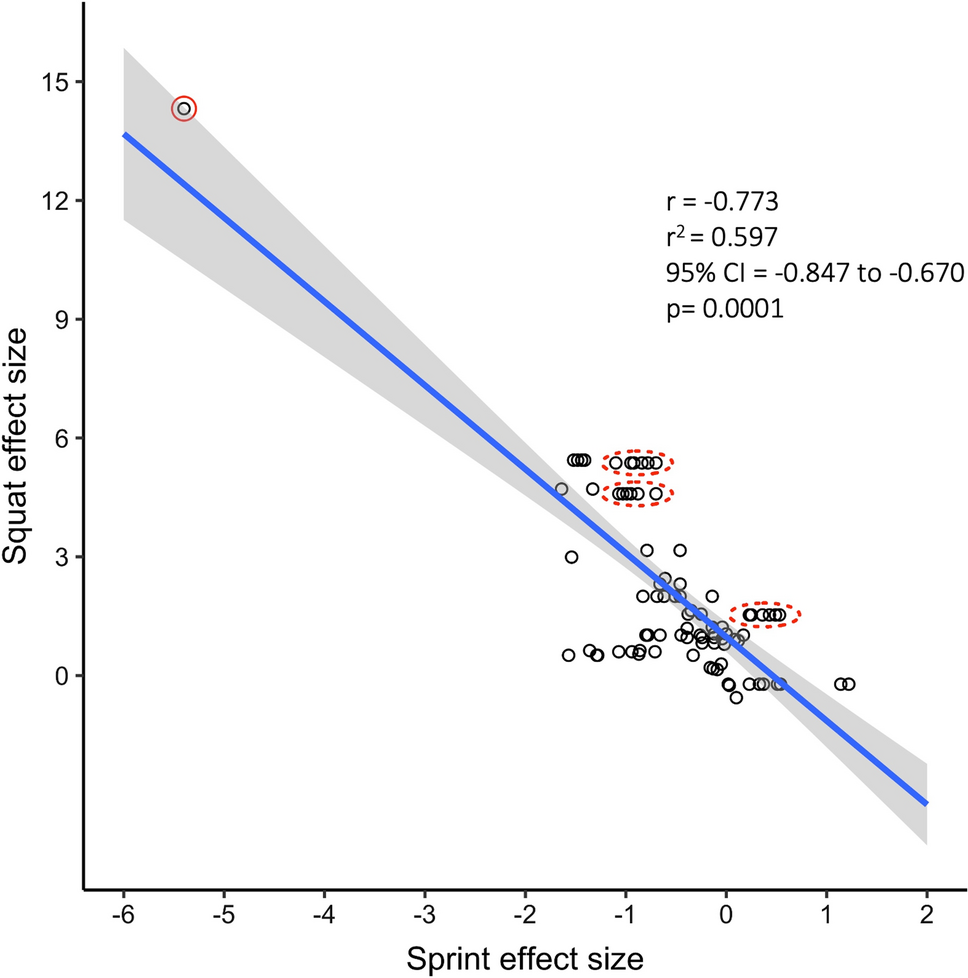
\includegraphics[width=\textwidth]{img/sd_vs_se/kadlec_effect_size.png}
    \caption*{ The most severe over-estimation of effect size made by \href{https://doi.org/10.1007/s40279-014-0227-1}{Seitz et al. (2014)} was for \href{https://doi.org/10.1519/JSC.0b013e3181aa36a2}{Wong et al. (2010)} (solid red circle in the upper right corner of this plot). \href{https://doi.org/10.1007/s40279-022-01766-0}{Kadlec et al. (2022)} corrected the statistical errors made by Seitz et al., finding that Seitz et al. had dramatically overestimated the correlation between lower body strength training and improvement in sprinting performance as a result of these errors. Adapted from Figure 1 of Kadlec et al.}
\end{figure}

\pagebreak

\subsection*{Example 2: Over-weighting studies in a meta-analysis due to using standard error instead of standard deviation}

\href{https://doi.org/10.1016/j.ijcrp.2023.200232}{Garg et al. (2024)} performed a meta-analysis to assess whether the systolic blood pressure was different for groups performing breathing exercises versus not performing breathing exercises at baseline (i.e. before any intervention was applied; note that there is no logical reason to perform this comparison, as it gives no information on the effectiveness of the intervention, but this meta-analysis has numerous issues that are beyond the scope of this guide). For at least two studies, \href{https://doi.org/10.3389/fphys.2020.00898}{Fetter et al. (2020)} and \href{https://doi.org/10.1161/JAHA.121.020980}{Craighead et al. (2021)}, the authors include the standard error as reported by these studies instead of the standard deviation, resulting in these studies being weighted far too heavily.

\begin{figure}[h!tbp]
    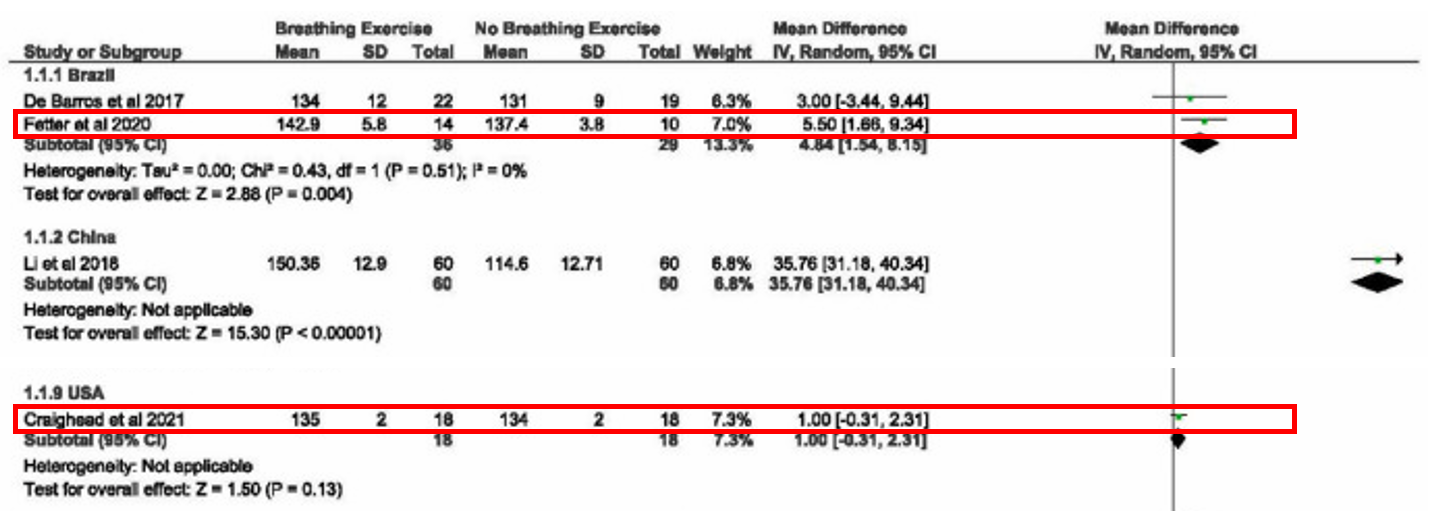
\includegraphics[width=\textwidth]{img/sd_vs_se/garg_problem.PNG}
    \caption*{\href{https://doi.org/10.1016/j.ijcrp.2023.200232}{Garg et al. (2024)} overweighted \href{https://doi.org/10.3389/fphys.2020.00898}{Fetter et al. (2020)} and \href{https://doi.org/10.1161/JAHA.121.020980}{Craighead et al. (2021)} (highlighted in their forest plot in red boxes) as a result of confusing standard error for standard deviation. As a result, Fetter et al. and Craighead et al. are each weighted greater than Li et al. (2018) which had three to four times as many participants. Adapted from Figure 2 of Garg et al.}
\end{figure}

\subsection*{Example 3: Over-weighting studies in a meta-analysis due to using standard error instead of standard deviation}

\href{https://doi.org/10.1007/s11882-023-01085-y}{Chagas et al. (2023)} performed a meta-analysis to determine whether treatment with the drug \href{https://en.wikipedia.org/wiki/Tezepelumab}{tezepelumab} reduced asthma patients' scores on the \href{http://www.qoltech.co.uk/acq.html}{Asthma Control Questionnaire-6 (ACQ-6)}. For the \href{https://doi.org/10.1056/NEJMoa2034975}{NAVIGATOR trial}, the authors entered the reported standard error as the standard deviation, leading to this trial being weighted to 97.6\% for this outcome (meaning that this portion of the meta-analysis was almost entirely based on the results of the NAVIGATOR trial).

\begin{figure}[h!tbp]
    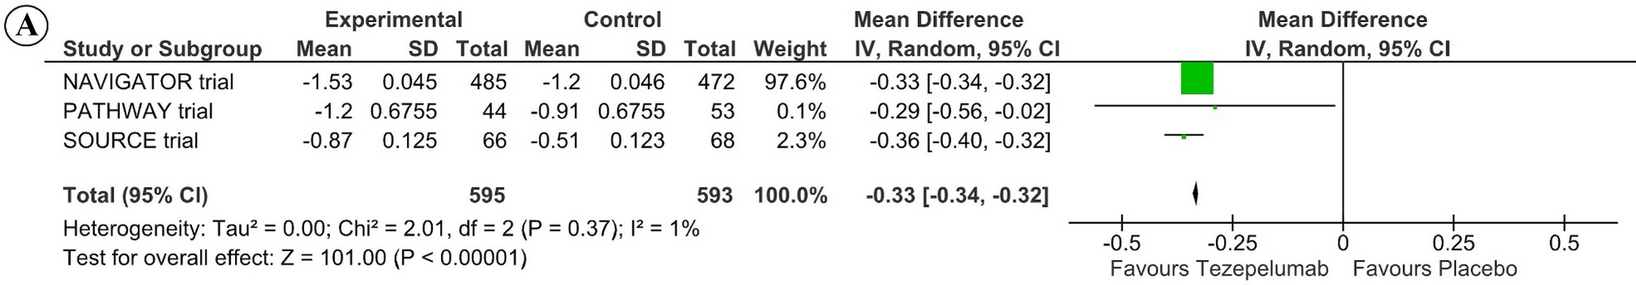
\includegraphics[width=\textwidth]{img/sd_vs_se/chagas_problem.png}
    \caption*{\href{https://doi.org/10.1007/s11882-023-01085-y}{Chagas et al. (2023)} overweighted the \href{https://doi.org/10.1056/NEJMoa2034975}{NAVIGATOR trial} as a result of confusing standard error for standard deviation. Note that the ``standard deviation'' reported in the above forest plot is much lower for the NAVIGATOR trial than the PATHWAY trial or the SOURCE trial. Adapted from Figure 2 of Chagas et al.}
\end{figure}

\pagebreak

\subsection*{Additional resources}

\begin{itemize}
    \setlength\itemsep{-0.5em}
    \item \href{https://doi.org/10.1038/nmeth.2659}{``Points of significance: Error bars'' (2013)}
    \item \href{https://doi.org/10.1007/s40279-023-01989-9}{``The Standard Error/Standard Deviation Mix-Up: Potential Impacts on Meta-Analyses in Sports Medicine'' (2024)}
    \item \href{https://doi.org/10.1007/s40279-022-01766-0}{``With Great Power Comes Great Responsibility: Common Errors in Meta-Analyses and Meta-Regressions in Strength \& Conditioning Research'' (2022)}
    \item \href{https://training.cochrane.org/handbook/current/}{\textit{The Cochrane Handbook for Systematic Reviews of Interventions}}
    \item \href{https://training.cochrane.org/handbook-diagnostic-test-accuracy/current}{\textit{The Cochrane Handbook for Systematic Reviews of Diagnostic Test Accuracy}}

\end{itemize}

% \setlength\itemsep{-0.5em}
% for bullet points and numbered lists.

\end{document}